\chapter{Raspberry Pi 5}
Jedná se o jednodeskový počítač, který je určen pro široké spektrum aplikací od IoT, rozpoznáváni obrazu, strojového učení, robotiku až po multimediální aplikace. Mezi hlavní výhody patří nízká cena, malé provozní náklady, možná modularita přes GPIO piny, PCI expres a USB porty a velkým množstvím tzv. HAT modulů, které jsou určeny pro rozšíření funkcí. \cite{Raspberry Pi 5}.

Pro tuto aplikaci bylo zvoleno Raspberry Pi 5 s 16 GB RAM, pamětí 256 GB a operačním systémem Raspberry Pi OS, který je stavěn na Linuxové distribuci Debianu. Hlavním důvodem výběru byla nízká cena, ale i jednoduchá dostupnost pro případného zájemce o domácí automatizaci, který by si chtěl systém ovládání a vizualizace vytvořit sám.

Jediným závažnějším problémem totoho zařízení je "obrušování" paměťové karty na které je nahrán operační systém. Tento problém je způsoben častým zápisem, který postupně snižuje životnost, rychlost a velikost paměti. V krajních případech i může dojít k úplnému zničení a ztrátě dat. K zamezení tohoto problému se historicky používala technika \textit{wear leveling} - rozložení zápisu na celou paměťovou kartu, aby se snížil počet zápisů na jednotlivé buňky \cite{wear leveling}. Teď už je možné použít M.2 NVMe SSD disk, který je připojen přes PCI expres a je mnohem rychlejší než paměťová karta. Tento disk je možné použít i jako bootovací disk, což zamezí problémům s bootováním a ztrátou dat. Další možností jak zpomalit toto obrušování je připojení USB flash disku, který za obětování rychlosti dokáže zamezit opotřebování paměti díky přenesení souborů s vyšší frekvencí zápisu - v tomto případě databáze.
\begin{figure}[!ht]
    \begin{center}
        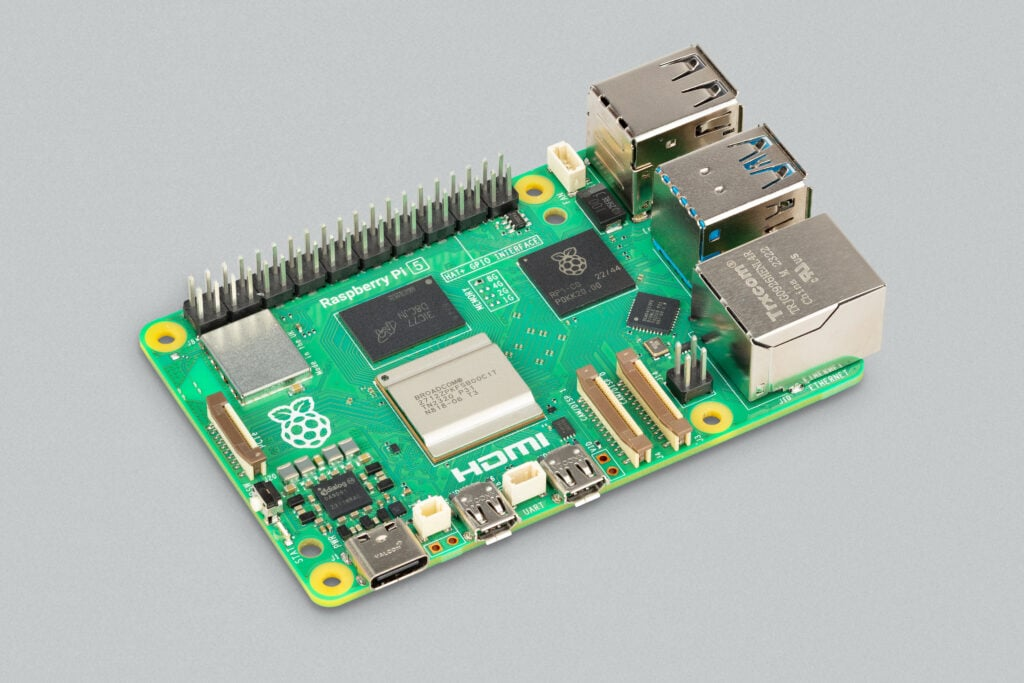
\includegraphics[scale=0.30]{obrazky/RaspberryPi5.jpg}
    \end{center}
    \caption[Raspberry Pi5 \cite{Raspberry Pi 5}]{Raspberry Pi5 \cite{Raspberry Pi 5}}
    \label{fig:RaspberryPi}
\end{figure}
\newpage
Alternativou k Raspberry Pi 5 můžou být LattePanda, ASUS NUC a podobné mikropočítače, které mají větší výkon, větší možnost výběru operačního systému (dostatečný výkon na Windows) a robustnost. Tyto výhody jsou kompenzovány vyšší pořizovací cenou, spotřebou a velikostí.
\section{Docker Compose}
Docker Compose je nástroj pro definici a správu více kontejnerových aplikací. Umožňuje uživatelům definovat aplikaci pomocí \textit{YAML} souboru, které obsahují informace o kontejnerových službách, sítích a uložištích. \cite{Docker Compose}

Instalace Docker Compose je jednoduchá a rozepsaná na oficiálních stránkách Dockeru. Obsahuje pouze tři kroky, které jsou již připravené pro kopírování do terminálu. \cite{DockerInstallationForDebian}

\subsection{Kontejnerizace}
Kontejnerizace je způsob virzualizace aplikací, které umožňuje spouštět v izolovaném prostředí s garancí funkčnosti v jakémkoliv prostředí, založený na linuxové technologii LXC (Linux Containers). Tento způsob je výhodný pro nasazení aplikací, které mají různé závislosti a konfigurace. Umožňuje také snadné nasazení a škálování aplikací. Dále tento způsob virtualizace dodávat kompletní prostředí, jako jiné virtuální stroje, ale s menšími režijními nároky na výkon a paměť, které přichází s fungováním separátního kernelu a simulací veškerého hardware. \cite{ContainerAndVirtualization}
V případě této práce byl navrhnut Docker Stack, který je složený z několika kontejnerů, které spolu komunikují a vytváří tak komplexní systém na ovládání a vizualizaci domácí automatizace. Vzhled tohoto stacku i s komunikacemi je zobrazen na Obr. \ref{fig:DockerStack}.
\begin{figure}[!ht]
    \begin{center}
        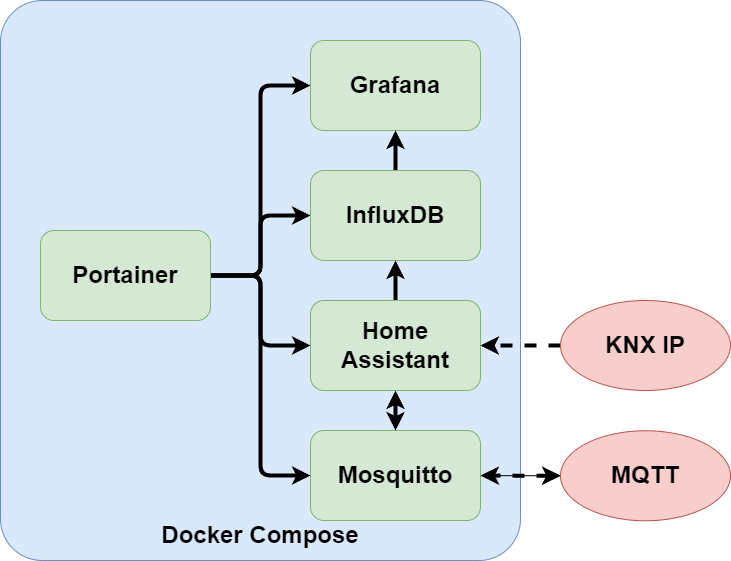
\includegraphics[scale=0.30]{obrazky/stack.png}
    \end{center}
    \caption[Docker Stack]{Docker Stack }
    \label{fig:DockerStack}
\end{figure}
\subsection{Tvorba YAML souboru}
YAML soubor je textový soubor, který obsahuje definici kontejnerů a jejich konfigurací. Je napsán v jazyce YAML (YAML Ain't Markup Language), což je formát pro serializaci dat \cite{YAML}. Níže je příklad vzhledu YAML souboru (Výpis \ref{lst:yaml}), který by měl pomoci ke snadnému pochopení struktury a syntaxe \cite{ComposeYamlExample}.

Dále pak může YAML soubor obsahovat i enviromentální proměnné, které se používají k nastavení kontejneru. Tyto proměnné mouhou být obsaženy v souboru .env, který se používá k uchování citlivých informací, jako jsou hesla a API klíče. Tento soubor je načítán při spuštění kontejneru. \cite{ENV}
\begin{lstlisting}[language=yaml, caption=Ukazka YAML souboru, label=lst:yaml]
version: "3" # Verze Docker Compose
services: # Sluzby
    name_of_service: # Jmeno sluzby
        image: name_of_image:latest # Jmeno image
        container_name: name_of_container # Jmeno kontejneru
        networks: # Site
            - name_of_network # Jmeno site na ktere pobezi kontejner
        depends_on: # Zavislosti
            - name_of_service # Jmeno kontejneru na kterem zavisi
        environment: # Promenne prostredi
        - PUID=1000 # ID uzivatele, ktery bude mit pristup k souborum
        - PGID=1000 # ID skupiny, ktera bude mit pristup k souborum
        - TZ=Europe/Prague # Casove pasmo
        - WEBUI_PORT=1234 # Port na kterem pobezi webove rozhrani 
        - DOCKER_MODS="linuxserver/mods:universal" # Docker modifikace
        volumes: # Slozky, ktere budou pripojeny do kontejneru
            - "/path/on/host:/path/in/container" # Cesta k souborum
        ports: # Porty pro pripojeni k hostitelske site
            - "host_port:container_port"
        deploy: # Nasazeni kontejneru
            resources:
                limits:
                    memory: 512m # Maximalni pamet
                    cpus: "1" # Maximalni CPU
                reservations:
                    memory: 256m # Minimalni pamet
                    cpus: "0.5" # Minimalni CPU
        restart: always # Restart kontejneru pri padu
        labels: # Metada
            - "com.docker.compose.project=project_name" # Nazev projektu
            - "com.docker.compose.service=service_name" # Nazev sluzby
            - "com.docker.compose.version=1.0" # Verze sluzby
\end{lstlisting}
\noindent Celková implementace je v přílohách \ref{apend:portainer} a \ref{apend:stackyaml}.
\subsection{Portainer}
Jedná se o open-source kontejner, který slouží jako webové rozhraní pro správu Dockeru. Umožňuje uživatelům spravovat kontejnery, Image, Stacky, Sítě, Uložiště, čtení logů, sledování výkonu, správa portů a další funkce. Jednou z předních výhod je jednoduchost použití kromě rozhraní je i propojení s Docker Hubem, což je veřejná knihovna kontejnerů. \cite{Portainer} 
\section{Mosquitto}
\section{Home Assistant}
\section{Influxdb}
\section{Grafana}